% Created by tikzDevice version 0.10.1 on 2018-01-31 10:28:46
% !TEX encoding = UTF-8 Unicode
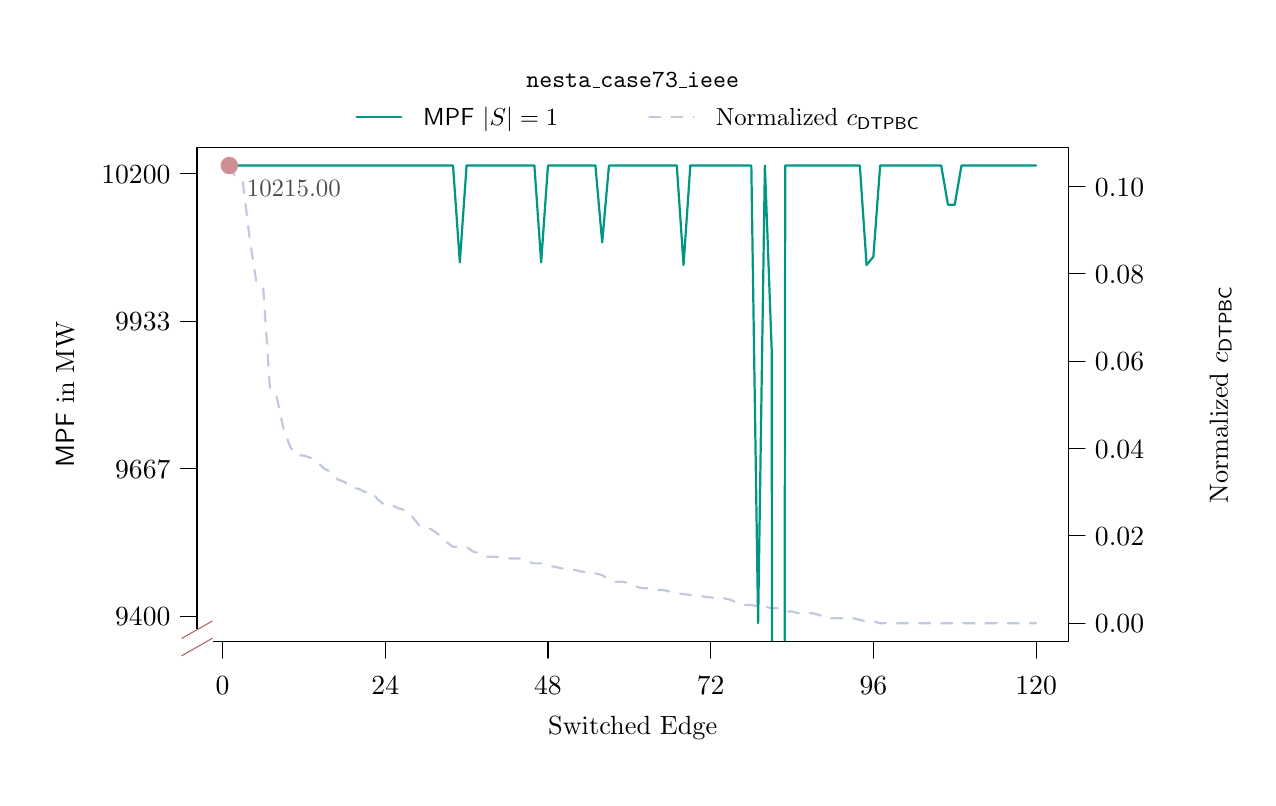
\begin{tikzpicture}[x=1pt,y=1pt]
\definecolor{fillColor}{RGB}{255,255,255}
\path[use as bounding box,fill=fillColor,fill opacity=0.00] (0,0) rectangle (440.85,271.01);
\begin{scope}
\path[clip] (  0.00,  0.00) rectangle (440.85,271.01);
\definecolor{drawColor}{RGB}{193,202,220}

\path[draw=drawColor,line width= 0.8pt,dash pattern=on 4pt off 4pt ,line join=round,line cap=round] ( 72.86,221.20) --
	( 75.31,216.69) --
	( 77.76,215.19) --
	( 80.21,194.78) --
	( 82.66,178.88) --
	( 85.11,177.07) --
	( 87.56,140.46) --
	( 90.01,137.46) --
	( 92.46,126.05) --
	( 94.91,119.45) --
	( 97.36,116.45) --
	( 99.81,116.45) --
	(102.26,115.54) --
	(104.71,114.04) --
	(107.16,111.64) --
	(109.61,110.44) --
	(112.06,107.74) --
	(114.51,106.84) --
	(116.96,104.74) --
	(119.41,104.44) --
	(121.86,103.24) --
	(124.31,103.24) --
	(126.76,100.24) --
	(129.21, 98.44) --
	(131.66, 98.44) --
	(134.11, 97.24) --
	(136.56, 96.64) --
	(139.01, 94.23) --
	(141.46, 91.23) --
	(143.90, 90.63) --
	(146.35, 89.43) --
	(148.80, 87.63) --
	(151.25, 85.23) --
	(153.70, 83.43) --
	(156.15, 83.43) --
	(158.60, 83.43) --
	(161.05, 81.63) --
	(163.50, 81.03) --
	(165.95, 79.83) --
	(168.40, 79.83) --
	(170.85, 79.83) --
	(173.30, 79.23) --
	(175.75, 79.23) --
	(178.20, 79.23) --
	(180.65, 78.03) --
	(183.10, 77.43) --
	(185.55, 77.43) --
	(188.00, 76.53) --
	(190.45, 76.23) --
	(192.90, 75.63) --
	(195.35, 75.63) --
	(197.80, 75.02) --
	(200.25, 74.42) --
	(202.70, 74.42) --
	(205.15, 73.82) --
	(207.60, 73.22) --
	(210.05, 71.42) --
	(212.50, 70.82) --
	(214.95, 70.82) --
	(217.40, 70.22) --
	(219.85, 69.02) --
	(222.30, 68.42) --
	(224.75, 68.42) --
	(227.20, 67.82) --
	(229.65, 67.82) --
	(232.10, 67.22) --
	(234.55, 66.62) --
	(237.00, 66.32) --
	(239.45, 66.02) --
	(241.90, 66.02) --
	(244.35, 65.42) --
	(246.80, 65.12) --
	(249.25, 64.82) --
	(251.70, 64.82) --
	(254.15, 64.22) --
	(256.60, 63.02) --
	(259.05, 62.42) --
	(261.49, 62.42) --
	(263.94, 61.82) --
	(266.39, 61.82) --
	(268.84, 61.22) --
	(271.29, 61.22) --
	(273.74, 60.02) --
	(276.19, 60.02) --
	(278.64, 59.42) --
	(281.09, 59.42) --
	(283.54, 59.42) --
	(285.99, 58.82) --
	(288.44, 57.62) --
	(290.89, 57.62) --
	(293.34, 57.62) --
	(295.79, 57.62) --
	(298.24, 57.62) --
	(300.69, 57.02) --
	(303.14, 56.42) --
	(305.59, 56.42) --
	(308.04, 55.82) --
	(310.49, 55.82) --
	(312.94, 55.82) --
	(315.39, 55.82) --
	(317.84, 55.82) --
	(320.29, 55.82) --
	(322.74, 55.82) --
	(325.19, 55.82) --
	(327.64, 55.82) --
	(330.09, 55.82) --
	(332.54, 55.82) --
	(334.99, 55.82) --
	(337.44, 55.82) --
	(339.89, 55.82) --
	(342.34, 55.82) --
	(344.79, 55.82) --
	(347.24, 55.82) --
	(349.69, 55.82) --
	(352.14, 55.82) --
	(354.59, 55.82) --
	(357.04, 55.82) --
	(359.49, 55.82) --
	(361.94, 55.82) --
	(364.39, 55.82);
\end{scope}
\begin{scope}
\path[clip] (  0.00,  0.00) rectangle (440.85,271.01);
\definecolor{drawColor}{RGB}{0,0,0}

\path[draw=drawColor,line width= 0.4pt,line join=round,line cap=round] ( 61.20, 49.20) --
	(376.05, 49.20) --
	(376.05,227.81) --
	( 61.20,227.81) --
	( 61.20, 49.20);
\end{scope}
\begin{scope}
\path[clip] (  0.00,  0.00) rectangle (440.85,271.01);
\definecolor{drawColor}{RGB}{0,0,0}

\path[draw=drawColor,line width= 0.4pt,line join=round,line cap=round] (376.05, 55.82) -- (376.05,213.57);

\path[draw=drawColor,line width= 0.4pt,line join=round,line cap=round] (376.05, 55.82) -- (382.05, 55.82);

\path[draw=drawColor,line width= 0.4pt,line join=round,line cap=round] (376.05, 87.37) -- (382.05, 87.37);

\path[draw=drawColor,line width= 0.4pt,line join=round,line cap=round] (376.05,118.92) -- (382.05,118.92);

\path[draw=drawColor,line width= 0.4pt,line join=round,line cap=round] (376.05,150.47) -- (382.05,150.47);

\path[draw=drawColor,line width= 0.4pt,line join=round,line cap=round] (376.05,182.02) -- (382.05,182.02);

\path[draw=drawColor,line width= 0.4pt,line join=round,line cap=round] (376.05,213.57) -- (382.05,213.57);

\node[text=drawColor,anchor=base west,inner sep=0pt, outer sep=0pt, scale=  1.00] at (385.65, 52.37) {0.00};

\node[text=drawColor,anchor=base west,inner sep=0pt, outer sep=0pt, scale=  1.00] at (385.65, 83.92) {0.02};

\node[text=drawColor,anchor=base west,inner sep=0pt, outer sep=0pt, scale=  1.00] at (385.65,115.47) {0.04};

\node[text=drawColor,anchor=base west,inner sep=0pt, outer sep=0pt, scale=  1.00] at (385.65,147.03) {0.06};

\node[text=drawColor,anchor=base west,inner sep=0pt, outer sep=0pt, scale=  1.00] at (385.65,178.58) {0.08};

\node[text=drawColor,anchor=base west,inner sep=0pt, outer sep=0pt, scale=  1.00] at (385.65,210.13) {0.10};
\end{scope}
\begin{scope}
\path[clip] (  0.00,  0.00) rectangle (440.85,271.01);
\definecolor{drawColor}{RGB}{0,150,130}

\path[draw=drawColor,line width= 0.8pt,line join=round,line cap=round] (118.89,238.60) -- (134.91,238.60);
\definecolor{drawColor}{RGB}{193,202,220}

\path[draw=drawColor,line width= 0.8pt,dash pattern=on 4pt off 4pt ,line join=round,line cap=round] (224.63,238.60) -- (240.65,238.60);
\definecolor{drawColor}{RGB}{0,0,0}

\node[text=drawColor,anchor=base,inner sep=0pt, outer sep=0pt, scale=  0.89] at (218.62,249.28) {\texttt{nesta\_case73\_ieee}};

\node[text=drawColor,anchor=base west,inner sep=0pt, outer sep=0pt, scale=  0.89] at (142.92,235.54) {$\mathsf{MPF}~|S|=1$};

\node[text=drawColor,anchor=base west,inner sep=0pt, outer sep=0pt, scale=  0.89] at (248.66,235.54) {Normalized~$c_\mathsf{DTPBC}$};
\end{scope}
\begin{scope}
\path[clip] (  0.00,  0.00) rectangle (440.85,271.01);
\definecolor{drawColor}{RGB}{0,0,0}

\path[draw=drawColor,line width= 0.4pt,line join=round,line cap=round] ( 61.20, 58.32) -- ( 61.20,218.20);

\path[draw=drawColor,line width= 0.4pt,line join=round,line cap=round] ( 61.20, 58.32) -- ( 55.20, 58.32);

\path[draw=drawColor,line width= 0.4pt,line join=round,line cap=round] ( 61.20,111.61) -- ( 55.20,111.61);

\path[draw=drawColor,line width= 0.4pt,line join=round,line cap=round] ( 61.20,164.91) -- ( 55.20,164.91);

\path[draw=drawColor,line width= 0.4pt,line join=round,line cap=round] ( 61.20,218.20) -- ( 55.20,218.20);

\node[text=drawColor,anchor=base east,inner sep=0pt, outer sep=0pt, scale=  1.00] at ( 51.60, 54.88) {9400};

\node[text=drawColor,anchor=base east,inner sep=0pt, outer sep=0pt, scale=  1.00] at ( 51.60,108.17) {9667};

\node[text=drawColor,anchor=base east,inner sep=0pt, outer sep=0pt, scale=  1.00] at ( 51.60,161.46) {9933};

\node[text=drawColor,anchor=base east,inner sep=0pt, outer sep=0pt, scale=  1.00] at ( 51.60,214.76) {10200};
\end{scope}
\begin{scope}
\path[clip] (  0.00,  0.00) rectangle (440.85,271.01);
\definecolor{drawColor}{RGB}{255,255,255}
\definecolor{fillColor}{RGB}{255,255,255}

\path[draw=drawColor,line width= 0.4pt,line join=round,line cap=round,fill=fillColor] ( 55.69, 47.20) rectangle ( 66.71, 53.45);
\definecolor{drawColor}{RGB}{188,97,104}

\path[draw=drawColor,line width= 0.4pt,line join=round,line cap=round] ( 55.69, 44.08) -- ( 66.71, 50.33);

\path[draw=drawColor,line width= 0.4pt,line join=round,line cap=round] ( 55.69, 50.33) -- ( 66.71, 56.58);
\end{scope}
\begin{scope}
\path[clip] ( 61.20, 49.20) rectangle (376.05,227.81);
\definecolor{drawColor}{RGB}{0,150,130}

\path[draw=drawColor,line width= 0.8pt,line join=round,line cap=round] ( 72.86,221.20) --
	( 75.31,221.20) --
	( 77.76,221.20) --
	( 80.21,221.20) --
	( 82.66,221.20) --
	( 85.11,221.20) --
	( 87.56,221.20) --
	( 90.01,221.20) --
	( 92.46,221.20) --
	( 94.91,221.20) --
	( 97.36,221.20) --
	( 99.81,221.20) --
	(102.26,221.20) --
	(104.71,221.20) --
	(107.16,221.20) --
	(109.61,221.20) --
	(112.06,221.20) --
	(114.51,221.20) --
	(116.96,221.20) --
	(119.41,221.20) --
	(121.86,221.20) --
	(124.31,221.20) --
	(126.76,221.20) --
	(129.21,221.20) --
	(131.66,221.20) --
	(134.11,221.20) --
	(136.56,221.20) --
	(139.01,221.20) --
	(141.46,221.20) --
	(143.90,221.20) --
	(146.35,221.20) --
	(148.80,221.20) --
	(151.25,221.20) --
	(153.70,221.20) --
	(156.15,186.22) --
	(158.60,221.20) --
	(161.05,221.20) --
	(163.50,221.20) --
	(165.95,221.20) --
	(168.40,221.20) --
	(170.85,221.20) --
	(173.30,221.20) --
	(175.75,221.20) --
	(178.20,221.20) --
	(180.65,221.20) --
	(183.10,221.20) --
	(185.55,186.22) --
	(188.00,221.20) --
	(190.45,221.20) --
	(192.90,221.20) --
	(195.35,221.20) --
	(197.80,221.20) --
	(200.25,221.20) --
	(202.70,221.20) --
	(205.15,221.20) --
	(207.60,193.44) --
	(210.05,221.20) --
	(212.50,221.20) --
	(214.95,221.20) --
	(217.40,221.20) --
	(219.85,221.20) --
	(222.30,221.20) --
	(224.75,221.20) --
	(227.20,221.20) --
	(229.65,221.20) --
	(232.10,221.20) --
	(234.55,221.20) --
	(237.00,185.26) --
	(239.45,221.20) --
	(241.90,221.20) --
	(244.35,221.20) --
	(246.80,221.20) --
	(249.25,221.20) --
	(251.70,221.20) --
	(254.15,221.20) --
	(256.60,221.20) --
	(259.05,221.20) --
	(261.49,221.20) --
	(263.94, 55.82) --
	(266.39,221.20) --
	(268.84,154.73) --
	(269.04,  0.00);

\path[draw=drawColor,line width= 0.8pt,line join=round,line cap=round] (273.48,  0.00) --
	(273.74,221.20) --
	(276.19,221.20) --
	(278.64,221.20) --
	(281.09,221.20) --
	(283.54,221.20) --
	(285.99,221.20) --
	(288.44,221.20) --
	(290.89,221.20) --
	(293.34,221.20) --
	(295.79,221.20) --
	(298.24,221.20) --
	(300.69,221.20) --
	(303.14,185.26) --
	(305.59,188.24) --
	(308.04,221.20) --
	(310.49,221.20) --
	(312.94,221.20) --
	(315.39,221.20) --
	(317.84,221.20) --
	(320.29,221.20) --
	(322.74,221.20) --
	(325.19,221.20) --
	(327.64,221.20) --
	(330.09,221.20) --
	(332.54,207.05) --
	(334.99,207.05) --
	(337.44,221.20) --
	(339.89,221.20) --
	(342.34,221.20) --
	(344.79,221.20) --
	(347.24,221.20) --
	(349.69,221.20) --
	(352.14,221.20) --
	(354.59,221.20) --
	(357.04,221.20) --
	(359.49,221.20) --
	(361.94,221.20) --
	(364.39,221.20);
\end{scope}
\begin{scope}
\path[clip] ( 61.20, 49.20) rectangle (376.05,227.81);
\definecolor{fillColor}{RGB}{207,142,147}

\path[fill=fillColor] ( 72.86,221.20) circle (  3.15);
\end{scope}
\begin{scope}
\path[clip] ( 61.20, 49.20) rectangle (376.05,227.81);
\definecolor{drawColor}{gray}{0.30}

\node[text=drawColor,anchor=base,inner sep=0pt, outer sep=0pt, scale=  0.90] at ( 96.18,210.04) {10215.00};
\end{scope}
\begin{scope}
\path[clip] (  0.00,  0.00) rectangle (440.85,271.01);
\definecolor{drawColor}{RGB}{0,0,0}

\path[draw=drawColor,line width= 0.4pt,line join=round,line cap=round] ( 70.41, 49.20) -- (364.39, 49.20);

\path[draw=drawColor,line width= 0.4pt,line join=round,line cap=round] ( 70.41, 49.20) -- ( 70.41, 43.20);

\path[draw=drawColor,line width= 0.4pt,line join=round,line cap=round] (129.21, 49.20) -- (129.21, 43.20);

\path[draw=drawColor,line width= 0.4pt,line join=round,line cap=round] (188.00, 49.20) -- (188.00, 43.20);

\path[draw=drawColor,line width= 0.4pt,line join=round,line cap=round] (246.80, 49.20) -- (246.80, 43.20);

\path[draw=drawColor,line width= 0.4pt,line join=round,line cap=round] (305.59, 49.20) -- (305.59, 43.20);

\path[draw=drawColor,line width= 0.4pt,line join=round,line cap=round] (364.39, 49.20) -- (364.39, 43.20);

\node[text=drawColor,anchor=base,inner sep=0pt, outer sep=0pt, scale=  1.00] at ( 70.41, 30.00) {0};

\node[text=drawColor,anchor=base,inner sep=0pt, outer sep=0pt, scale=  1.00] at (129.21, 30.00) {24};

\node[text=drawColor,anchor=base,inner sep=0pt, outer sep=0pt, scale=  1.00] at (188.00, 30.00) {48};

\node[text=drawColor,anchor=base,inner sep=0pt, outer sep=0pt, scale=  1.00] at (246.80, 30.00) {72};

\node[text=drawColor,anchor=base,inner sep=0pt, outer sep=0pt, scale=  1.00] at (305.59, 30.00) {96};

\node[text=drawColor,anchor=base,inner sep=0pt, outer sep=0pt, scale=  1.00] at (364.39, 30.00) {120};

\node[text=drawColor,anchor=base,inner sep=0pt, outer sep=0pt, scale=  0.95] at (218.62, 15.60) {Switched Edge};

\node[text=drawColor,rotate= 90.00,anchor=base,inner sep=0pt, outer sep=0pt, scale=  0.95] at ( 16.80,138.51) {$\mathsf{MPF}$ in~$\mathrm{MW}$};

\node[text=drawColor,rotate= 90.00,anchor=base,inner sep=0pt, outer sep=0pt, scale=  0.95] at (433.65,138.51) {Normalized~$c_\mathsf{DTPBC}$};
\end{scope}
\end{tikzpicture}
